% TEX compiler = latexmk
% copyright arturo salinas-aguayo 2024
\documentclass[12pt]{article}

\usepackage{graphicx}
\usepackage{amsmath}
\usepackage{array}
\usepackage{amsfonts}
\usepackage{fancyhdr}
\usepackage{geometry}
\usepackage{circuitikz}
\usepackage{subfigure}
\usepackage{caption}
\usepackage{karnaugh-map}
\usepackage{bm}
\usepackage{float}

\geometry{letterpaper, margin=1in}
\graphicspath{ {../images/} }

% Header and Footer
\pagestyle{fancy}
\fancyhf{}
\fancyhead[L]{CSE 2301 - Lab 07: Hamming Code}
\fancyhead[R]{\thepage}
\setlength{\headheight}{15pt}

\author{Arturo Salinas-Aguayo}
\title{Lab 07: Hamming Code}
% theorem set
\newtheorem{example}{Example}
% Example block environment
\newenvironment{examp}
{\vspace{0.5cm}
 \hrule
\vspace{0.5cm}
\begin{example}}
{\hrule
\vspace{0.5cm}
\end{example}}

\begin{document}
\newcommand{\closure}[2][3]{%
	{}\mkern#1mu\overline{\mkern-#1mu#2}}
\newcommand\ncoverline[1]{\mkern1mu\overline{\mkern-1mu#1\mkern-1mu}\mkern1mu}
% Title Page
\begin{titlepage}
	\centering
	\vspace*{3cm}
	\huge\textbf{Lab 07: Hamming Code}\\
	\vspace{5cm}
	\Large\textbf{Arturo Salinas-Aguayo}\\
	\normalsize
	CSE 2301: Principles and Practice of Digital Logic Design\\
	Dr. Mohammad Khan, Section 003L-1248\\
	Electrical and Computer Engineering Department
	\vfill
	
\includegraphics[scale=0.1]{uconnlogo}\\
	College of Engineering, University of Connecticut\\
	\scriptsize{Coded in \LaTeX}
	\vspace*{1cm}
\end{titlepage}
\section*{Theory}
\subsection*{The Hamming Code}
In order to properly describe what is going on, I must define a few key terms of importance:
\begin{itemize}
	\item \textbf{Dataword}: The dataword is the original data that is to be transmitted.
	\item \textbf{Codeword}: The codeword is the dataword with the parity bits added to it.
	\item \textbf{Parity Bit}: A parity bit is a bit added to the dataword to ensure that the data is transmitted correctly. In this context, we assume "even" parity, meaning that the number of 1's in the dataword plus the parity bit is even.
\end{itemize}

In a Hamming code, each position in the codeword corresponds to a unique binary identifier, allowing specific parity bits to cover particular data bits. By observing which parity bits fail, we can determine the position of an erroneous bit. The following table summarizes how failing parity bits reveal the error location and provide guidance for correction:

\begin{table}[h!]
	\centering
	\renewcommand{\arraystretch}{1.3}
	\begin{tabular}{|c|c|c|}
		\hline
		\textbf{Parity Failures} & \textbf{Error Position (Binary)} & \textbf{Correction}    \\
		\hline
		None                     & 000                              & No correction needed   \\
		\hline
		\( P_1 \)                & 001                              & Flip bit at position 1 \\
		\hline
		\( P_2 \)                & 010                              & Flip bit at position 2 \\
		\hline
		\( P_1, P_2 \)           & 011                              & Flip bit at position 3 \\
		\hline
		\( P_4 \)                & 100                              & Flip bit at position 4 \\
		\hline
		\( P_1, P_4 \)           & 101                              & Flip bit at position 5 \\
		\hline
		\( P_2, P_4 \)           & 110                              & Flip bit at position 6 \\
		\hline
		\( P_1, P_2, P_4 \)      & 111                              & Flip bit at position 7 \\
		\hline
	\end{tabular}
	\caption{Hamming Code Error Detection and Correction Table}
\end{table}
\begin{itemize}
	\item Each bit position is associated with a unique binary representation that aligns with specific failing parity checks.
	\item Failing parity bits correspond to powers of 2: \( P_1 \) (1), \( P_2 \) (2), and \( P_4 \) (4).
	\item By observing which parity bits fail, we form a binary code that indicates the exact location of the erroneous bit.
\end{itemize}

This approach allows precise detection and correction of single-bit errors, ensuring data integrity during transmission. This is implemented in Part 2 of the lab during the Error Position Identification step.
\subsection*{Hamming Distance?}
So, what exactly is Hamming distance? In my research, including reading from Richard W. Hamming’s book \textit{The Art of Doing Science and Engineering: Learning to Learn}, Hamming distance is a metric for measuring how many bit positions differ between two strings of the same length. It provides a way to quantify the distance between symbols in a binary space. In the context of error detection and correction, Hamming distance determines how many errors can be detected and corrected in a data stream.

According to Hamming, the properties of the distance metric can be described by standard conditions, such as non-negativity, identity, symmetry, and the triangle inequality. These characteristics allow us to effectively analyze the relationships between codewords:

In error-correcting codes, the minimum Hamming distance between valid codewords is essential to the code’s ability to correct and detect errors:

\begin{itemize}
	\item A minimum Hamming distance of 1 provides unique identification but no ability to detect errors.
	\item A distance of 2 allows single-bit error detection.
	\item A distance of 3 enables single-bit error correction, as the erroneous code remains within the radius of 1 from the original codeword.
	\item A distance of 4 provides a balance that enables single-bit error correction and double-bit error detection.
\end{itemize}
\subsection*{Logic for Double Error Detection}
As Hamming puts it, a minimum hamming  distance of 4 will allow us to implement this. To detect double errors in a Hamming code, we add an overall parity bit \( P_0 \) to the codeword. This parity bit checks the parity of the entire codeword, including both data and parity bits.
\[
	P_0 = D_1 \oplus D_2 \oplus D_4 \oplus D_8 \oplus P_1 \oplus P_2 \oplus P_4
\]
where:
\begin{itemize}
	\item \( D_1, D_2, D_4, D_8 \): Data bits in the Hamming code.
	\item \( P_1, P_2, P_4 \): Existing parity bits positioned at powers of 2 in the Hamming code.
\end{itemize}
\[
	\text{If } P_0 = 1 \text{, a double error may have occurred.}
\]
\begin{itemize}
	\item \textbf{Single Error}: If there is only a single-bit error, the standard Hamming code error-correction mechanism (using \( P_1 \), \( P_2 \), and \( P_4 \)) will identify and correct it. In this case, \( P_0 \) will still satisfy the expected parity.
	\item \textbf{Double Error}: If two bits are in error, \( P_0 \) will detect this inconsistency by indicating an unexpected parity, signaling a double error in the data.
\end{itemize}
In this configuration, the addition of \( P_0 \) allows the system to detect but not correct double errors, thereby increasing the reliability of the transmitted data.
\subsection*{Required Parity Bits for Hamming Code}
In a Hamming code, the required number of parity bits \( p \) for \( m \) data bits must satisfy the inequality:
\[
	2^p \geq m + p + 1
\]
This inequality ensures that the code has sufficient redundancy to detect and correct errors. The positions for the parity bits follow a pattern based on powers of 2, such as 1, 2, 4, 8, and so on. This pattern suggests that as the number of data bits increases, the number of required parity bits also increases logarithmically.
\subsubsection*{Graph of Parity Bits Required}
The following graph illustrates the relationship between the number of data bits and the required parity bits for values of \( m \) ranging from 4 to 67. Each step represents when an additional parity bit is necessary.


\centerline{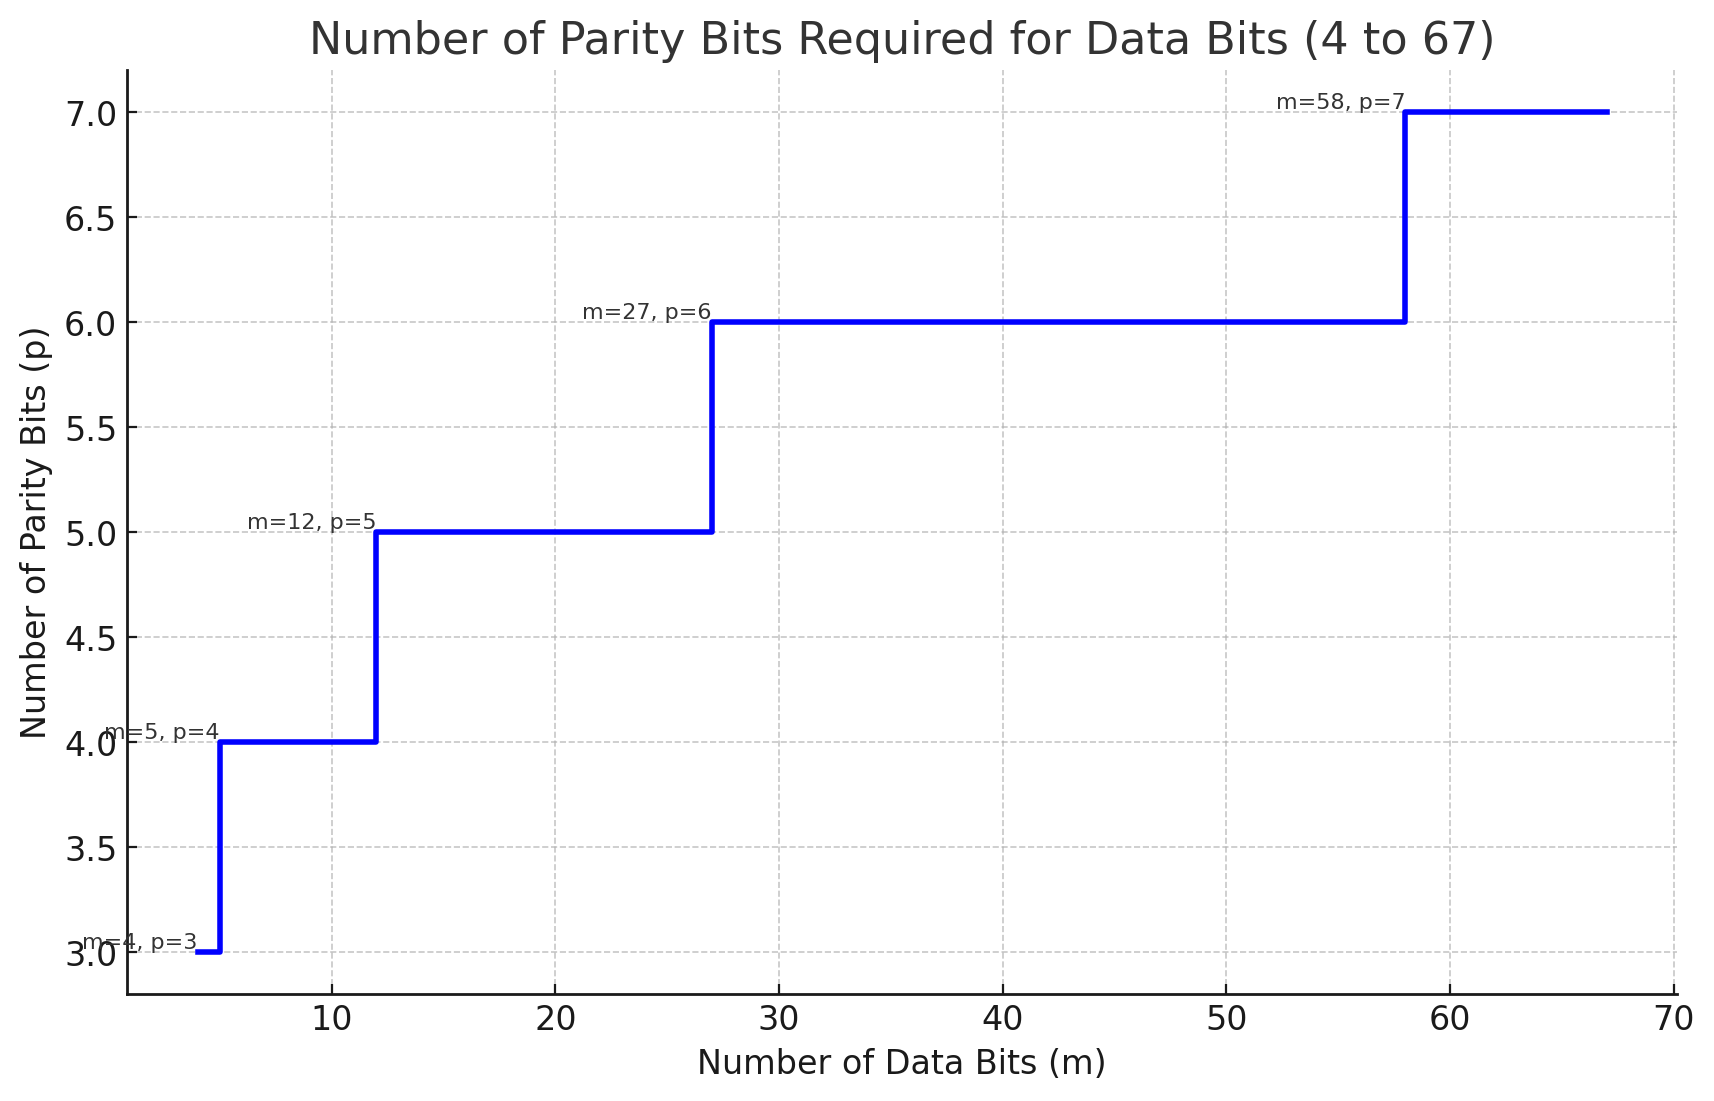
\includegraphics[scale=0.65]{examp071}}
We see our first point is at \(m = 4\) and \(p = 3\), which is the minimum number of parity bits required to detect and correct single-bit errors. As the number of data bits increases, the number of parity bits also increases to maintain the minimum Hamming distance necessary for error correction.

The next is at \(m = 5\) and \(p = 4\), which is the minimum number of parity bits required to detect and correct double-bit errors.
The rest are
\begin{itemize}
	\item \(m = 12\) and \(p = 5\)
	\item \(m = 27\) and \(p = 6\)
	\item \(m = 58\) and \(p = 7\)
\end{itemize}
\subsection*{Discussion}
To conclude, the Hamming code is a powerful error-correcting code that can detect and correct single-bit errors and detect double-bit errors. The code’s ability to correct errors is based on the minimum Hamming distance between valid codewords, which is determined by the number of parity bits added to the dataword. By increasing the redundancy of the code, the Hamming code can effectively detect and correct errors in data transmission, ensuring the integrity of the message. The implementation was way simpler

A dive into Hamming's work reveals the elegance and simplicity of his approach to error detection and correction, which has become a cornerstone of modern coding theory. His insights into the properties of the Hamming distance and the importance of parity bits have paved the way for the development of more sophisticated error-correcting codes that are used in various applications today.

While his work does get in the weeds fast, reading through his book, \textit{The
	Art of Doing Science and Engineering: Learning to Learn}, provides a fascinating
look at the thought process and methodology behind his groundbreaking
contributions to coding theory. His emphasis on learning from mistakes,
embracing challenges, and thinking creatively resonates with anyone seeking to
push the boundaries of knowledge and innovation and a joy to read.

The next pracice questions explore more parity and timing diagrams in which a
propogation delay is introduced and explored in combinational logic.

Looking forward, this will get way more complicated once the logic depends on a
rising or falling edge to trigger the data to be passed, cleared, or preset.

\section*{Practice Questions} \begin{examp} \textbf{Timing Diagram for Given
		Circuit}\\ For the given diagram, we are given that the INV gate has a
	propagation delay of \(3 ns\) and the AND and OR gates have a \(5 ns\) delay.
	We are also told of our 4 inputs, \(A, B, C, D\) \[ A = 0 \quad B = 1 \quad C
		= 0 \quad D = 0 \] The question proposes that after \(4 ns\), \(A\) flips to
	high, which sets off a "chain reaction" called a transport delay which
	propogates through the circuit as drawn in the following timing diagram.
	\centerline{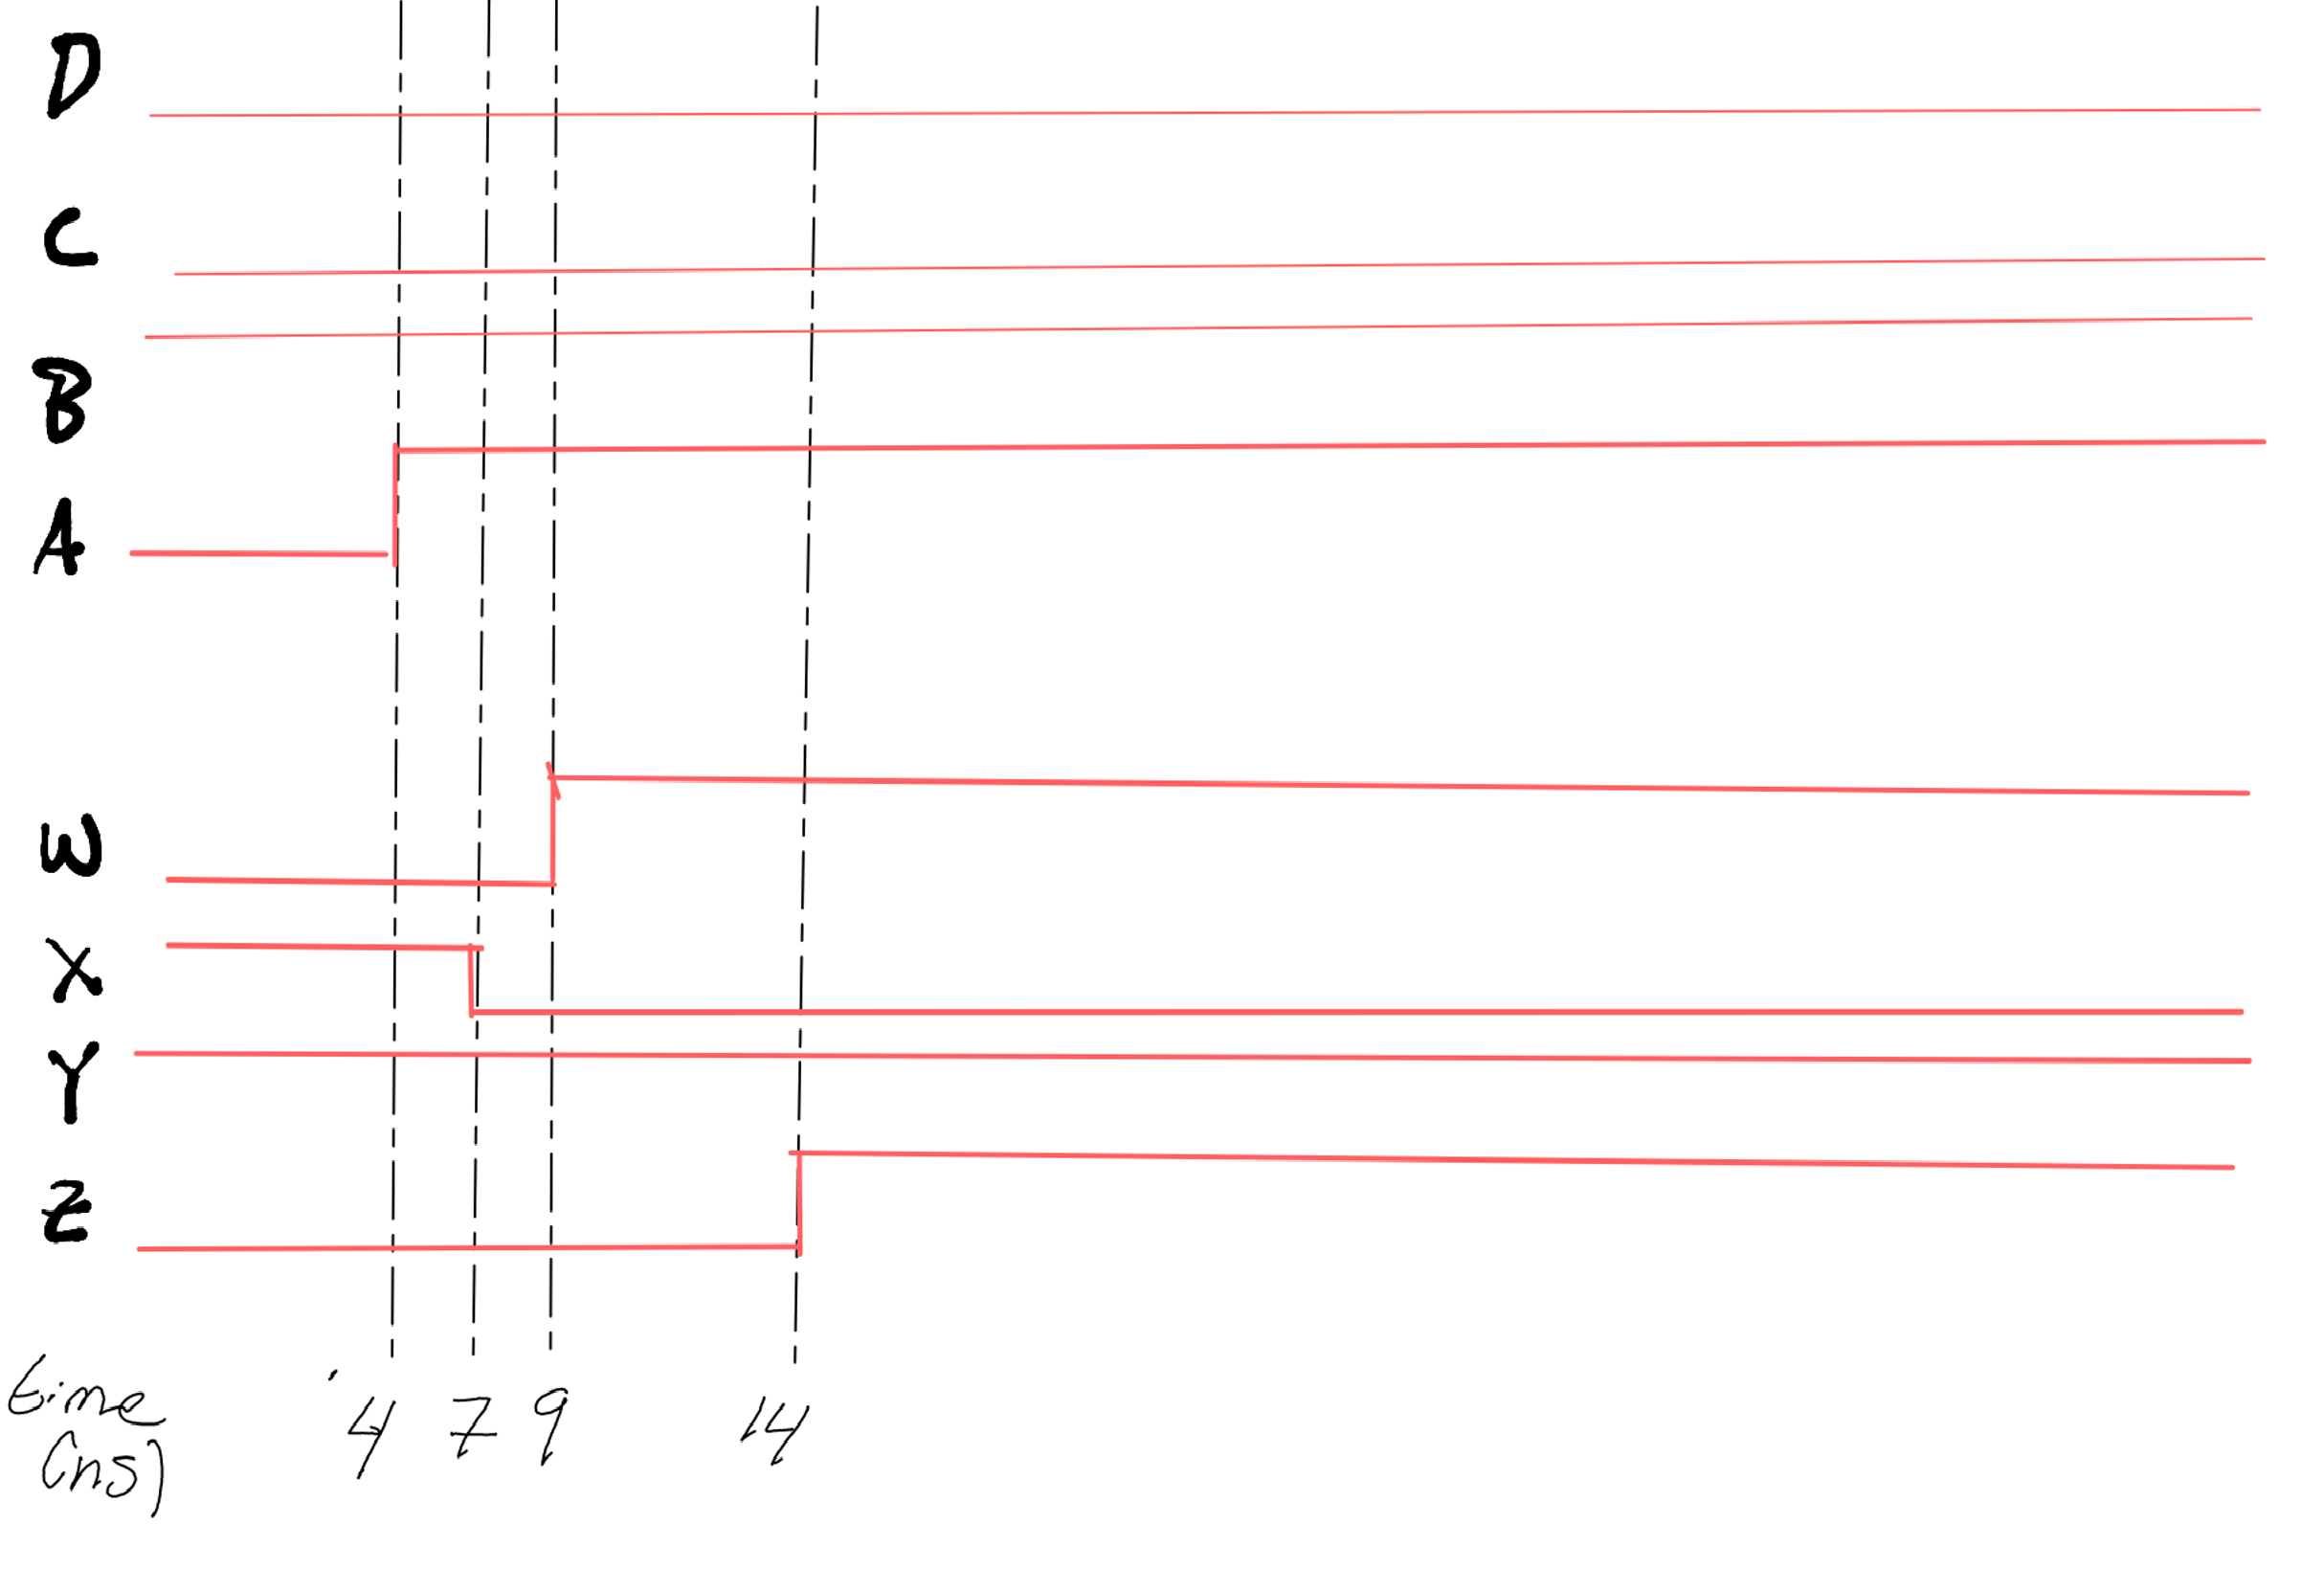
\includegraphics[scale=0.45]{examp072}} \end{examp}

\begin{examp} \textbf{Completing an Odd Parity Table}\\ Odd parity ensures the
	total number of 1's in the codeword is odd, while even parity ensures the
	total number of 1's is even.

	To complete the Hamming code table, we calculated the required parity bits for
	each 4-bit hex value, ensuring odd parity for each parity bit.

	\begin{itemize} \item \textbf{Hex 0} (Binary: 0000): All parity bits \( P_1
		      \), \( P_2 \), and \( P_4 \) are set to 0 to maintain odd parity. \item
		      \textbf{Hex 6} (Binary: 0110): The calculated values for \( P_1 = 0 \), \(
		      P_2 = 1 \), and \( P_4 = 1 \) ensure odd parity for each parity check group.
		\item \textbf{Hex B} (Binary: 1011): The values \( P_1 = 1 \), \( P_2 = 0 \),
		      and \( P_4 = 1 \) achieve odd parity for each check group. \end{itemize}

	The completed table is as follows:

	\begin{center} \begin{tabular}{|c|c|c|c|c|c|c|c|} \hline \textbf{Hex} & \( P_1
               \)                                      & \( P_2 \) & \( P_3 \) & \( P_4 \) & \( P_5 \) & \( P_6 \) & \( P_7 \) \\
               \hline
               0                                       & 0         & 0         & 0         & 0         & 0         & 0
                                                       & 0                                                                     \\
               6                                       & 0         & 1         & 1         & 1         & 0         & 1
                                                       & 0                                                                     \\ B            & 1         & 0         & 1
                                                       & 1         & 0         & 1         & 1                                 \\ \hline
		\end{tabular} \end{center} The binary representation of hex B is \(1011\).
	Placing the data bits in positions \( P_3 \), \( P_5 \), \( P_6 \), and \( P_7
	\), we have: \[ P_1 \quad P_2 \quad 1 \quad P_4 \quad 0 \quad 1 \quad 1 \] The
	parity bits are calculated as follows: \begin{itemize} \item \( P_1 \) checks
		      bits \( P_1 \), \( P_3 \), \( P_5 \), and \( P_7 \) (bits: \( P_1 \), 1, 0,
		      1). To achieve odd parity, we set \( P_1 = 1 \). \item \( P_2 \) checks bits
		      \( P_2 \), \( P_3 \), \( P_6 \), and \( P_7 \) (bits: \( P_2 \), 1, 1, 1).
		      To maintain odd parity, we set \( P_2 = 0 \). \item \( P_4 \) checks bits \(
		      P_4 \), \( P_5 \), \( P_6 \), and \( P_7 \) (bits: \( P_4 \), 0, 1, 1). To
		      achieve odd parity, we set \( P_4 = 1 \). \end{itemize}

	Thus, the final 7-bit code for hex B is: \[
		1 \quad 0 \quad 1 \quad 1 \quad 0 \quad 1 \quad 1 \] \end{examp}
\begin{examp} \textbf{Logic for Odd Parity}\\ As stated before, Odd Parity
	simply means that the data bits and the parity bit add up to an odd
	number. This is very similar to our implementation in the lab, however
	we can simply NOT (or take the inverse) of the general operation to
	obtain the correct logic.

	Recall that the \(\oplus\) operation is the XOR operation and it
	operates similar to a bitwise addition without carry. To generate an odd
	parity bit from four data bits \( A \), \( B \), \( C \), and \( D \),
	we can use the following logic expression: \[			\text{Odd Parity} =
		\overline{A \oplus B \oplus C \oplus D}\]

\end{examp} \begin{examp} \textbf{Correcting a 7-bit Hamming Code with
		Even Parity}\\ Given: \[ P_1 = 1, \quad P_2 = 0, \quad P_3 = 0, \quad
		P_4 = 0, \quad P_5 = 1, \quad P_6 = 1, \quad P_7 = 1 \] In a 7-bit
	Hamming code, positions \( P_1 \), \( P_2 \), and \( P_4 \) are parity
	bits. Each parity bit checks specific data bit positions to maintain
	even parity just like the lab: \begin{itemize} \item \textbf{\( P_1 \)}
		      checks bits \( P_1 \), \( P_3 \), \( P_5 \), and \( P_7 \): \[ P_1 =
			      1, \quad P_3 = 0, \quad P_5 = 1, \quad P_7 = 1 \] Sum: \( 1 + 0 + 1 +
		      1 = 3 \) (odd) \\ Since the sum is odd, this parity check
		      \textbf{fails.}

		\item \textbf{\( P_2 \)} checks bits \( P_2 \), \( P_3 \), \( P_6 \),
		      and \( P_7 \): \[ P_2 = 0, \quad P_3 = 0, \quad P_6 = 1, \quad P_7 =
			      1 \] Sum: \( 0 + 0 + 1 + 1 = 2 \) (even) \\ This parity check
		      passes.

		\item \textbf{\( P_4 \)} checks bits \( P_4 \), \( P_5 \), \( P_6 \),
		      and \( P_7 \): \[ P_4 = 0, \quad P_5 = 1, \quad P_6 = 1, \quad P_7 = 1
		      \] Sum: \( 0 + 1 + 1 + 1 = 3 \) (odd) \\ Since the sum is odd, this
		      parity check \textbf{fails.} \end{itemize} Since parity checks \( P_1 \) and
	\( P_4 \) failed while \( P_2 \) passed, we add the positions of the failing
	parity bits to determine the position of the erroneous bit: \[ P_1 + P_4 = 1
		+ 4 = 5 \] Thus, the erroneous bit is at \textbf{position 5}. To correct the
	code, we flip the bit at position 5: \[ \textbf{Original code: } 1, 0, 0, 0,
		1, 1, 1 \] \[ \textbf{Corrected code: } 1, 0, 0, 0, 0, 1, 1 \] \end{examp}
\begin{examp} \textbf{Finding values from an Odd Triangular Code}\\ Find
	the values for all the check/parity bits in the following odd triangular
	code. Each check bit \( C_i \) should ensure that the total number of
	1's in its row is odd. \[ \begin{array}{|ccccccc|c|} \hline
			1 & 0   & 0   & 0   & 0   & 1          & C_1 & C_1 = \, ? \\
			0 & 1   & 0   & 1   & 1   & C_2        &     & C_2 = \, ? \\
			1 & 0   & 1   & 0   & C_3 &            &     & C_3 = \, ? \\
			1 & 1   & 0   & C_4 &     &            &     & C_4 = \, ? \\
			0 & 1   & C_5 &     &     &            &     & C_5 = \, ? \\
			0 & C_6 &     &     &     &            &     & C_6 = \, ? \\ C_7 &     &
			  &     &     &     &     & C_7 = \, ?                    \\ \hline\end{array} \]
	\begin{enumerate} \item \textbf{Calculating \( C_1 \)}: \\ Row: \( 1,
		      0, 0, 0, 0, 1 \) \\ Sum of 1's without \( C_1 \): \( 1 + 0 + 0 + 0 +
		      0 + 1 = 2 \) (even) \\ Since we need odd parity, set \( C_1 = 1 \).

		\item \textbf{Calculating \( C_2 \)}: \\ Row: \( 0, 1, 0, 1, 1 \) \\
		      Sum of 1's without \( C_2 \): \( 0 + 1 + 0 + 1 + 1 = 3 \) (odd) \\
		      Since the sum is already odd, set \( C_2 = 0 \).

		\item \textbf{Calculating \( C_3 \)}: \\ Row: \( 1, 0, 1, 0 \) \\
		      Sum of 1's without \( C_3 \): \( 1 + 0 + 1 + 0 = 2 \) (even) \\ To
		      make it odd, set \( C_3 = 1 \).

		\item \textbf{Calculating \( C_4 \)}: \\ Row: \( 1, 1, 0 \) \\ Sum
		      of 1's without \( C_4 \): \( 1 + 1 + 0 = 2 \) (even) \\ To achieve
		      odd parity, set \( C_4 = 1 \).

		\item \textbf{Calculating \( C_5 \)}: \\ Row: \( 0, 1 \) \\ Sum of
		      1's without \( C_5 \): \( 0 + 1 = 1 \) (odd) \\ Since the sum is
		      already odd, set \( C_5 = 0 \).

		\item \textbf{Calculating \( C_6 \)}: \\ Row: \( 0 \) \\ Sum of 1's
		      without \( C_6 \): \( 0 \) (even) \\ To make it odd, set \( C_6 =
		      1 \).

		\item \textbf{Calculating \( C_7 \)}: \\ Row: (only \( C_7 \)) \\ To
		      ensure odd parity by default, set \( C_7 = 1 \). \end{enumerate}
	\textbf{Final Table:} \[ \begin{array}{|ccccccc|c|} \hline
			1 & 0 & 0 & 0 & 0 & 1 & 1 & C_1 = 1 \\
			0 & 1 & 0 & 1 & 1 & 0 &   & C_2 = 0 \\
			1 & 0 & 1 & 0 & 1 &   &   & C_3 = 1 \\
			1 & 1 & 0 & 1 &   &   &   & C_4 = 1 \\
			0 & 1 & 0 &   &   &   &   & C_5 = 0 \\
			0 & 1 &   &   &   &   &   & C_6 = 1 \\
			1 &   &   &   &   &   &   & C_7 = 1 \\ \hline\end{array} \]
\end{examp} \end{document}
% vim: set ft=tex tw=80 ts=2 sts=2 sw=2 noet:
